\documentclass[12pt, a4paper]{report}
\usepackage[top=1cm, left=1cm, right=1cm]{geometry}

\usepackage[utf8]{inputenc}
\usepackage[russian]{babel}

\usepackage{array}
\newcolumntype{M}[1]{>{\centering\arraybackslash}m{#1}}

\usepackage{hyperref}
\hypersetup{
	colorlinks,
	citecolor=black,
	filecolor=black,
	linkcolor=black,
	urlcolor=black
}

\usepackage{sectsty}
\allsectionsfont{\centering}

\usepackage{indentfirst}
\setlength\parindent{24pt}

\usepackage{algorithm}
\usepackage[noend]{algpseudocode}

\usepackage{listings}
\usepackage{xcolor}
\definecolor{codegreen}{rgb}{0,0.6,0}
\definecolor{codegray}{rgb}{0.5,0.5,0.5}
\definecolor{codepurple}{rgb}{0.58,0,0.82}
\definecolor{backcolour}{rgb}{0.95,0.95,0.92}
\lstdefinestyle{mystyle}{
    backgroundcolor=\color{backcolour},   
    commentstyle=\color{codegreen},
    keywordstyle=\color{magenta},
    numberstyle=\normalsize\color{codegray},
    stringstyle=\color{codepurple},
    basicstyle=\ttfamily\footnotesize,
    breakatwhitespace=false,         
    breaklines=true,                 
    captionpos=b,                    
    keepspaces=true,                 
    numbers=left,                    
    numbersep=5pt,                  
    showspaces=false,                
    showstringspaces=false,
    showtabs=false,                  
    tabsize=2
}

\usepackage{graphicx}
\graphicspath{{plots/pictures/}}

\begin{document}
	\begin{titlepage}
		\begin{center}
			\large \textbf{Министерство науки и высшего образования Российской Федерации} \\
			\large \textbf{Федеральное государственное бюджетное образовательное учреждение высшего образования} \\
			\large \textbf{«Российский химико-технологический университет имени Д.И. Менделеева»} \\

			\vspace*{4cm}
			\LARGE \textbf{ОТЧЕТ ПО ЛАБОРАТОРНОЙ РАБОТЕ №3}

			\vspace*{4cm}
			\begin{flushright}
				\Large
				\begin{tabular}{>{\raggedleft\arraybackslash}p{9cm} p{10cm}}
					Выполнил студент группы КС-36: & Золотухин А.А. \\
					Ссылка на репозиторий: & https://github.com/ \\
					& MUCTR-IKT-CPP/ \\
					& ZolotukhinAA\_36\_ALG \\
					Принял: & Крашенников Роман Сергеевич \\
					Дата сдачи: & 10.03.2025 \\
				\end{tabular}
			\end{flushright}

			\vspace*{6cm}
			\Large \textbf{Москва \\ 2025}
		\end{center}
	\end{titlepage}

	\tableofcontents
	\thispagestyle{empty}
	\newpage

	\pagenumbering{arabic}

	\section*{Описание задачи}
	\addcontentsline{toc}{section}{Описание задачи}
	\large
	Написать свою реализацию двусвязного списка:
	\begin{itemize}
		\item добавление элемента в начало, в конец, в произвольное место;
		\item удаление элемента из списка.
	\end{itemize}
	\par
	В рамках лабораторной работы необходимо изучить и реализовать двусвязный список. Структура должна:
	\begin{itemize}
		\item использовать шаблонный подход, обеспечивая работу контейнера с произвольными данными;
		\item реализовывать своё итератор, предоставляющий стандартный для языка механизм работы с ним (для \textit{C++} это операции \textit{++} и \textit{!=});
		\item обеспечивать работу стандартных библиотек и конструкции \textit{for each}, если она есть в языке, если их нет, то реализовать собственную функцию, использующую итератор;
		\item обеспечивать проверку на пустоту и подсчёт количества элементов.
	\end{itemize}
	\par
	Для демонстрации работы структуры необходимо создать набор тестов (под тестом понимается функция, которая создаёт структуру, проводит операцию или операции над структурой и удаляет структуру):
	\begin{itemize}
		\item заполнение контейнера \underline{1000} целыми числами в диапазоне от \underline{-1000} до \underline{1000} и подсчёт их суммы, среднего, минимального и максимального;
		\item провести проверку работы операций вставки и изъятия элементов на коллекции из \underline{10} строковых элементов;
		\item заполнение контейнера \underline{100} структур, содержащих фамилию, имя, отчество и дату рождения (от \underline{01.01.1980} до \underline{01.01.2020}). Значения каждого поля генерируются случайно из набора заранее заданных. После заполнения необходимо найти всех людей младше \underline{20} лет и старше \underline{30} и создать новые структуры, содержащие результат фильтрации, проверить выполнение на правильность подсчётом количества элементов, не подходящих под условие в новых структурах.
	\end{itemize}
	\par
	Тесты:
	\begin{enumerate}
		\item перемешать все элементы;
		\item выполнить серию тестирования сортировки из первой лабораторной на реализованном списке и сравнить производительность с полученной на массиве.
	\end{enumerate}

	\section*{Описание метода/модели}
	\addcontentsline{toc}{section}{Описание метода/модели}
	\large
	\textbf{Двусвязный список} - это двунаправленный список, в котором каждый узел имеет два указателя: на следующий и предыдущий узлы, которые ссылаются на следующий и предыдущий узлы соответственно. В отличие от односвязаного списка, в котором каждый узел указывает только на следующий узел, в двусвязном списке есть дополнительный предыдущий указатель, который позволяет перемещаться как вперёд, так и назад. \par
	Каждый узел двусвязного списка состоит из трёх полей:
	\begin{itemize}
		\item \textit{data} - значение, хранящееся в узле;
		\item \textit{next} - ссылка на следующий узел в списке;
		\item \textit{prev} - ссылка на предыдущий узел в списке.
	\end{itemize}
	\par
	Анализ сложности основных операций над двусвязным списком:
	\begin{itemize}
		\item \textbf{Вставка в начало}: \( O(1) \); 
		\item \textbf{Вставка в конец}: \( O(1) \); 
		\item \textbf{Вставка в опреденный узел}: \( O(n) \); 
		\item \textbf{Удаление в начале}: \( O(1) \); 
		\item \textbf{Удаление в конце}: \( O(1) \); 
		\item \textbf{Удаление в опреденном узле}: \( O(n) \); 
	\end{itemize}
	\par
	\textit{Преимущества}:
	\begin{itemize}
		\item Позволяет перемещаться как вперёд, так и назад;
		\item Удаление узла выполняется более эффективно и просто, поскольку у него есть указатель на предыдущий узел;
		\item Является динамическим по своей природе, поэтому он может увеличиваться и уменьшаться в размерах.
	\end{itemize}
	\par
	\textit{Недостатки}:
	\begin{itemize}
		\item Для каждого узла требуется больше памяти, чем для массивов, из-за дополнительного хранилища, используемого для указателей;
		\item Его сложнее реализовать и поддерживать по сравнению с односвязным списком;
		\item Нужно пройти от головного узла к определённому узлу для вставки и удаления в определённых местах.
	\end{itemize}

	\section*{Выполнение задачи}
	\addcontentsline{toc}{section}{Выполнение задачи}
	Двусвязный список реализован на языке \textit{C++}. Построение графиков с помощью программы \textit{GNUplot}.

	\textit{"main"} функция работает с вызовом методов для выполнения задания
	\lstset{style=mystyle}
	\begin{lstlisting}[language=C++]
		int main() {
			srand(time(0));

			testIntegers();
			testStrings();
			testPersons();
			testShuffle();
			simulation();

			return 0;
		}
	\end{lstlisting}
	\par
	\textit{"Node"} класс
	\lstset{style=mystyle}
	\begin{lstlisting}[language=C++]
		template <typename T>
		class Node {
			public:
				T data;
				Node<T> *prev;
				Node<T> *next;

				Node(const T &value) : data(value), prev(nullptr), next(nullptr) {}
		};
	\end{lstlisting}
	\par
	\textit{"LinkedList"} класс
	\lstset{style=mystyle}
	\begin{lstlisting}[language=C++]
		template <typename T>
		class LinkedList {
			protected:
				int size;
				Node<T> *head;
				Node<T> *tail;

			public:
				LinkedList() : size(0), head(nullptr), tail(nullptr) {}

				void insertFront(const T &value) {
					Node<T> *newNode = new Node<T>(value);
					if (head == nullptr) {
						head = newNode;
						tail = newNode;
					} else {
						newNode->next = head;
						head->prev = newNode;
						head = newNode;
					}
					
					size++;
				}

				bool isEmpty() const { return size == 0; }

				int getSize() const { return size; }

				class Iterator {
					private:
						Node<T> *current;

					public:
						Iterator(Node<T> *node) : current(node) {}

						T& operator*() const { return current->data; }

						Iterator& operator++() {
							if (current)
								current = current->next;

							return *this;
						}

						Iterator& operator--() {
							if (current)
								current = current->prev;

							return *this;
						}

						bool operator!=(const Iterator &other) const { return current != other.current; }
				};

				Iterator begin() const { return Iterator(head); }

				Iterator end() const { return Iterator(nullptr); }
		};
	\end{lstlisting}
	\par
	\textit{"DoublyLinkedList"} класс
	\lstset{style=mystyle}
	\begin{lstlisting}[language=C++]
		template <typename T>
		class DoublyLinkedList : public LinkedList<T> {
			public:
				void insertEnd(const T& value) {
					Node<T> *newNode = new Node<T>(value);
					if (this->head == nullptr) {
						this->head = newNode;
						this->tail = newNode;
					} else {
						newNode->prev = this->tail;
						this->tail->next = newNode;
						this->tail = newNode;
					}

					this->size++;
				}

				void insertAtPosition(const T &value, int position) {
					if (position < 0 || position > this->size)
						throw std::out_of_range("The position is out of range.");

					if (position == 0)
						this->insertFront(value);
					else if (position == this->size)
						this->insertEnd(value);
					else {
						Node<T> *newNode = new Node<T>(value);
						Node<T> *current = this->head;

						for (int i = 0; i < position - 1; i++)
							current = current->next;

						newNode->next = current->next;
						newNode->prev = current;
						current->next->prev = newNode;
						current->next = newNode;

						this->size++;
					}
				}

				void deleteNode(const T &value) {
					Node<T> *current = this->head;
					while (current != nullptr) {
						if (current->data == value) {
							if (current->prev != nullptr)
								current->prev->next = current->next;
							else
								this->head = current->next;

							if (current->next != nullptr)
								current->next->prev = current->prev;
							else
								this->tail = current->prev;
							
							delete current;

							this->size--;

							break;
						}

						current = current->next;
					}
				}

				void shuffle() {
					if (this->size <= 1)
						std::cerr << "There isn't anything to shuffle!";

					std::vector<T> elements;
					for (typename DoublyLinkedList<T>::Iterator it = this->begin(); it != this->end(); ++it)
						elements.push_back(*it);

					std::random_device rd;
					std::mt19937 gen(rd());
					std::shuffle(elements.begin(), elements.end(), gen);

					this->clear();
					for (const T &element : elements)
						this->insertEnd(element);
				}

				void clear() {
					while (this->head != nullptr) {
						Node<T>* temp = this->head;
						this->head = this->head->next;
						delete temp;
					}
					this->tail = nullptr;
					this->size = 0;
				}
		};
	\end{lstlisting}
	\par
	\textit{"testIntegers"} функция
	\lstset{style=mystyle}
	\begin{lstlisting}[language=C++]
		void testIntegers() {
			DoublyLinkedList<int> list;

			int sum = 0;
			int minValue = 1001;
			int maxValue = -1001;

			for (int i = 0; i < 1000; i++) {
				int value = getRandomNumber(-1000, 1000);
				list.insertEnd(value);
				sum += value;
				
				if (value < minValue) minValue = value;
				if (value < maxValue) maxValue = value;
			}

			double average = static\_cast<double>(sum) / list.getSize();

			std::cout << "Test: Integers" << std::endl;
			std::cout << "Sum: " << sum << std::endl;
			std::cout << "Average: " << average << std::endl;
			std::cout << "Min: " << minValue << std::endl;
			std::cout << "Max: " << maxValue << std::endl;
		}
	\end{lstlisting}

	\newpage
	\vfill

	\begin{figure}
		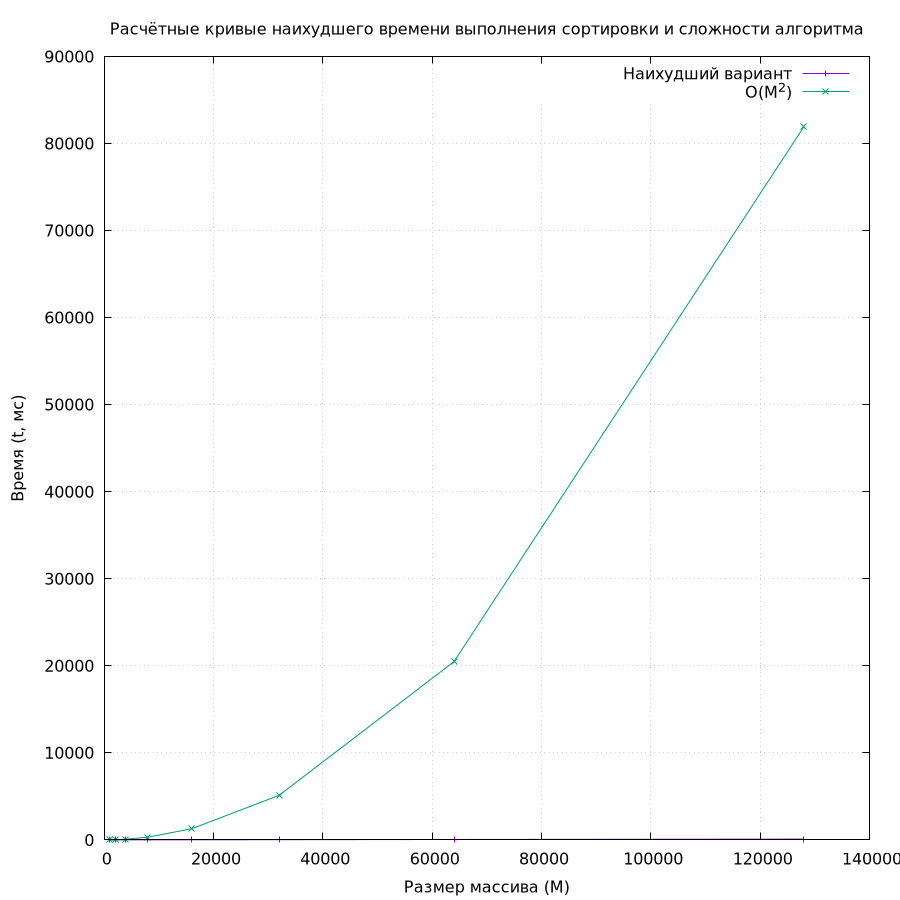
\includegraphics[width=300pt]{worst_and_complexity.png}
	\end{figure}
	\begin{figure}
		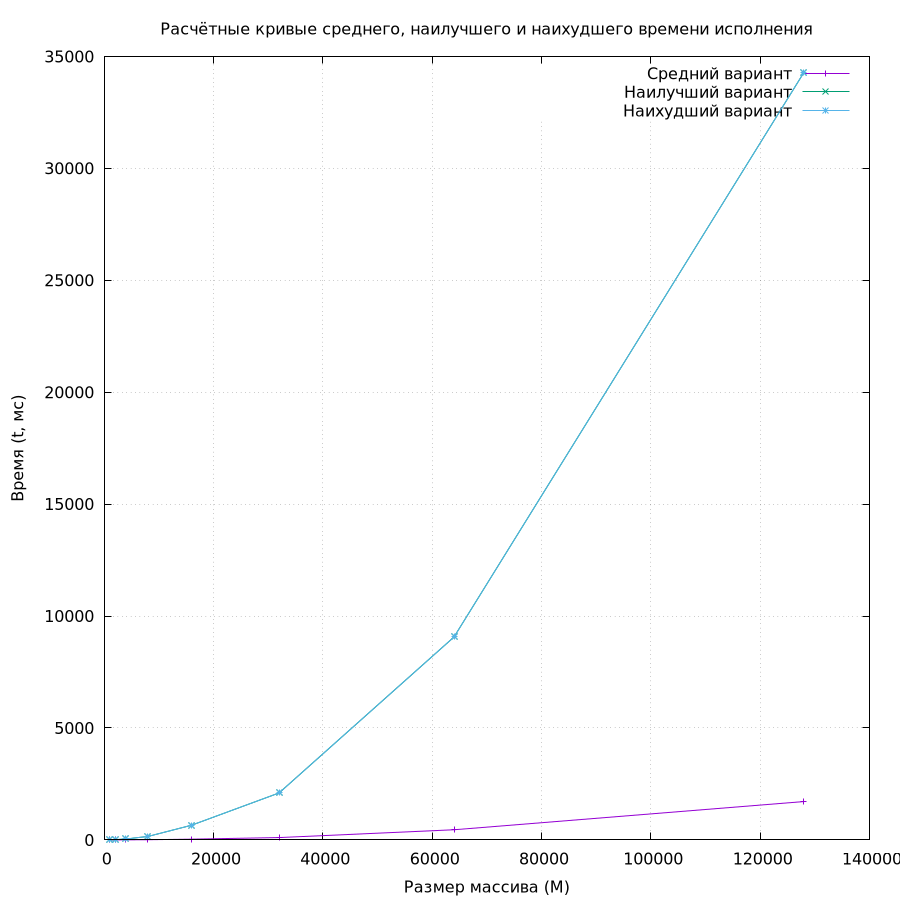
\includegraphics[width=300pt]{average_best_worst.png}
	\end{figure}
	\begin{figure}
		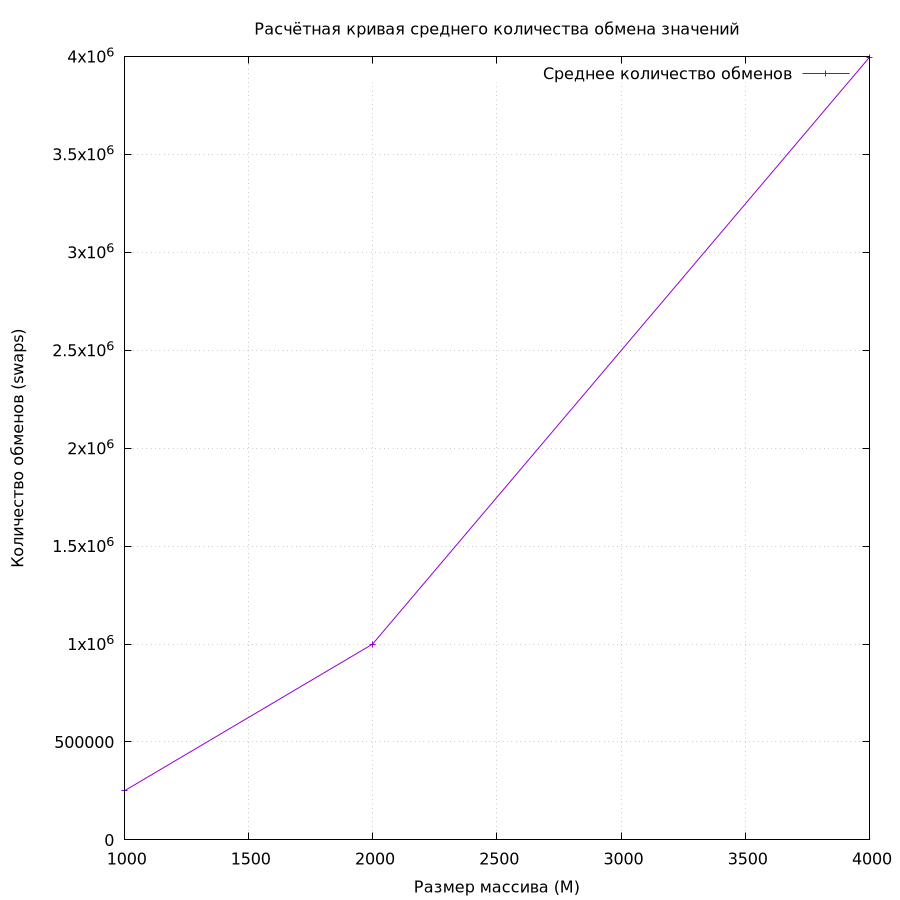
\includegraphics[width=300pt]{average_swaps.png}
	\end{figure}
	\begin{figure}
		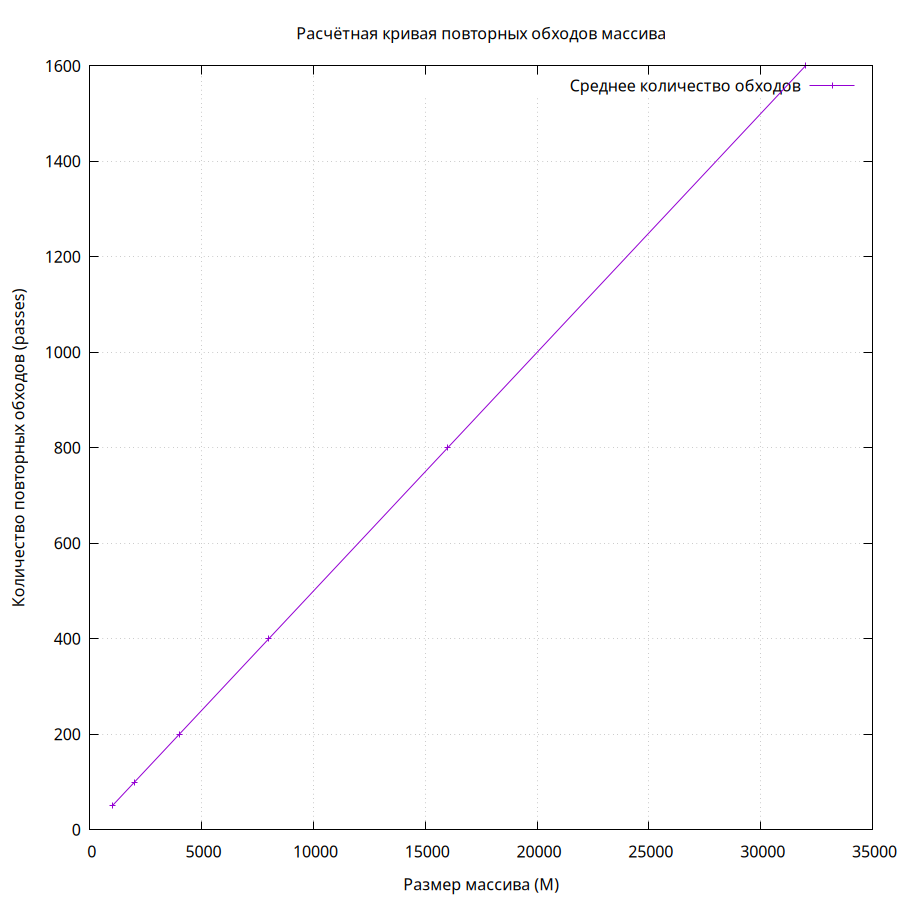
\includegraphics[width=300pt]{average_passes.png}
	\end{figure}

	\vfill
	\clearpage
	
	\section*{Выводы}
	\addcontentsline{toc}{section}{Выводы}
	Дву
\end{document}
